\documentclass[sigplan,10pt]{acmart}
\newcommand{\intraj}{\textsc{Intra}J}
\newcommand{\intracfg}{\textsc{IntraCFG}}
\newcommand{\extendj}{\textsc{Extend}J}
\newcommand{\magpie}{\textsc{Magpie Bridge}}
\newcommand{\jastadd}{\textsc{JastAdd}}
\newcommand{\code}[1]{\texttt{#1}}
\newcommand{\retType}[1]{{\color{red}#1}}
\usepackage{xargs}                     
\usepackage{xcolor}  
\usepackage{tabularx}
\usepackage{booktabs}
\usepackage{svg}
\usepackage{tikz}
\usepackage{hyperref}
\usepackage[colorinlistoftodos,prependcaption,textsize=tiny]{todonotes}
\usepackage[simplified]{pgf-umlcd}
\usepackage{xpatch} % Needed for patching pgf-umlcd
\usepackage{xparse} % Needed for patching pgf-umlcd
\usepackage{color,soul} % for \hl
\definecolor{dark-yellow}{RGB}{219, 212, 143}
\definecolor{dark-green}{RGB}{36,84,36}
\definecolor{my-gray}{gray}{0.85}
\sethlcolor{dark-yellow}
\usetikzlibrary{patterns,arrows,decorations.pathmorphing,backgrounds,shadows,positioning,fit,shapes,matrix,calc,shapes.multipart,arrows.meta}
\newcommandx{\idriss}[2][1=]{\todo[linecolor=blue,backgroundcolor=blue!25,bordercolor=blue,#1]{#2}}

\hypersetup{
    colorlinks=true,
    linkcolor=blue,
    filecolor=magenta,      
    urlcolor=cyan,
    }


\settopmatter{printfolios=true,printccs=false,printacmref=false}
%printfolios=true, means print page numbers
%printccs=false, means don't show CCS categories
%printacmref=false, means don't show acm reference


\acmConference[Course paper, EDAN70]{Project in computer science}{Lund University}{Sweden}
\acmYear{\today}

\startPage{1}

\setcopyright{none}

%% Bibliography style
\bibliographystyle{ACM-Reference-Format}

%Table columns
\newcolumntype{b}{X}
\newcolumntype{s}{>{\hsize=.5\hsize}X}

\begin{document}

%% Title information
\title[Efficient Code Fixes]{A Framework For Efficient Code Fixes Using Reference Attributed Grammars}         %% [Short Title] is optional;
                                        %% when present, will be used in
                                        %% header instead of Full Title.
%\subtitle{Subtitle}                     %% \subtitle is optional


%% Author information
%% Each author should be introduced by \author, followed by
%% \affiliation, and \email.

%% Author with single affiliation.
\author{Charlie Mrad}
\affiliation{
  \institution{D16, Lund University, Sweden}            %% \institution is required
}
\email{ch3045mr-s@student.lu.se}          %% \email is recommended

% \author{First2 Last2}
% \affiliation{
%   \institution{F13, Lund University, Sweden}            %% \institution is required
% }
% \email{name@domain}          %% \email is recommended


\begin{abstract}
Code fixes tools are essential for any developer and are often a feature of the more popular IDEs available today. They provide an efficient way for a programmer to learn potentially better ways to write their code and fix the potentially erroneous code automatically. The problem today comes from a lack of efficiency in how quickly the code fixes can be found and generated and how language analysing extensions for IDEs are being developed. This paper proposes a framework that can efficiently find potential errors in Java code using \intraj\ and provide quick-fix options. To avoid spending a significant amount of time implementing and maintaining LSP support for the framework \magpie\ is used. This combination provides a solid foundation to quickly provide an expandable array of code fixes. The initial evaluation seems to outperform Soot on a similar test case. There is still plenty of room for improvement on the proposed framework, but it appears to hold up reasonably well as a starting point.
\end{abstract}


\maketitle

\section{Introduction}
Static source code analysis provide helpful assistance in the software development process, allowing the programmer to detect critical problems, e.g., security flaws, run time errors, unintended behaviour. Recent studies \cite{tool_study1, tool_study2} have shown that the analysis needs to be responsive, evident in its feedback and results should be easy to access, i.e., collected in one central place, such as the integrated development environments (IDE). In this paper, the possibility of bringing the \intraj~\cite{intraj} framework for static analysis into IDEs is explored to improve the user experience when developing in Java.

\subsection{Introduction to \intraj}
\intraj\ is a control-flow analysis tool for the Java language that uses the language-independent framework \intracfg~\cite{intraj} to construct the control-flow graphs (CFGs). \intraj\ superimposes the CFGs on top of the Abstract Syntax Tree (AST) nodes of interest and is not tied to the underlying nested structure of the AST. Overall, \intraj\ provides an efficient and precise way of constructing CFGs for Java programs and can be used to create Java source code analyses. \intraj\ is built as an extension of the \extendj\ \cite{extendj} Java compiler. \extendj\ is written with \jastadd~\cite{jastadd} and uses the Reference Attributed Grammar formalism, enabling on-demand evaluation and declarative specification. This allows \extendj\ to be easily extended with new modules such as \intraj\ being a prime example. Similar to \extendj, \intraj is written using RAGs, meaning that the  analyses performed by \intraj\ are evaluated on-demand. Therefore, if an analysis is left unused, it does not have to be calculated and will not slow down the overall computation.\\ 
The static analyses \intraj\ provides can be a valuable tool for helping programmers during the development process, and while \intraj\ can provide useful information about analysis results it is all done through a command line interface. This is not ideal as the developer has to manually run commands as well as read through and match analysis results with the corresponding source code it refers too. That is where the Language Server Protocol (LSP) can come into play in order to facilitate the creation of extensions for IDEs and allow \intraj\ to display its results in the IDE text editor itself. This is accomplished by deferring the IDE features related to language support to external language-specific servers which communicate with the IDE according to LSP specifications \cite{lsp}.

\subsection{Introduction to \magpie}
While LSP does provide a manageable way to integrate language support into multiple IDEs without requiring IDE specific code, it does not eliminate the IDE integration work entirely. Many IDE extensions still suffer from a significant portion of the code base being dedicated to LSP communications which becomes especially evident for smaller projects which can sometimes only have as little as $\frac{1}{3}$ of the code dedicated to actual language analysis as illustrated in Table~\ref{lsp_overhead}. In order to attempt addressing this issue an LSP abstracting framework called \magpie\ was developed that allows users to simply set up their code to implement the \magpie\ interface and initialize an LSP server which in turn handles all the LSP communication for the extension \cite{magpie}.


\begin{table}[h!]
\begin{tabularx}{\columnwidth}{bccc}
\toprule
\textsc{Tool} & \textsc{Analysis} & \textsc{Plugin} & \textsc{Overhead} (\%)\\ 
\midrule
 \texttt{SPLift} & 1317 & 3317 & 71.6\\
 \texttt{CogniCrypt} & 11753 & 18766 & 61.5\\
  \texttt{PMD} & 117551 & 33435 & 22.1\\
\bottomrule
\end{tabularx}
 \caption{Brief table derived from Linghui Luo et al. paper on \magpie~\cite{magpie}. Shows the worst examples of LSP code overhead. The \textsc{Analysis} and \textsc{Plugin} are expressed in LoC.} 
 \label{lsp_overhead}
\end{table}

\begin{figure*}[t!]
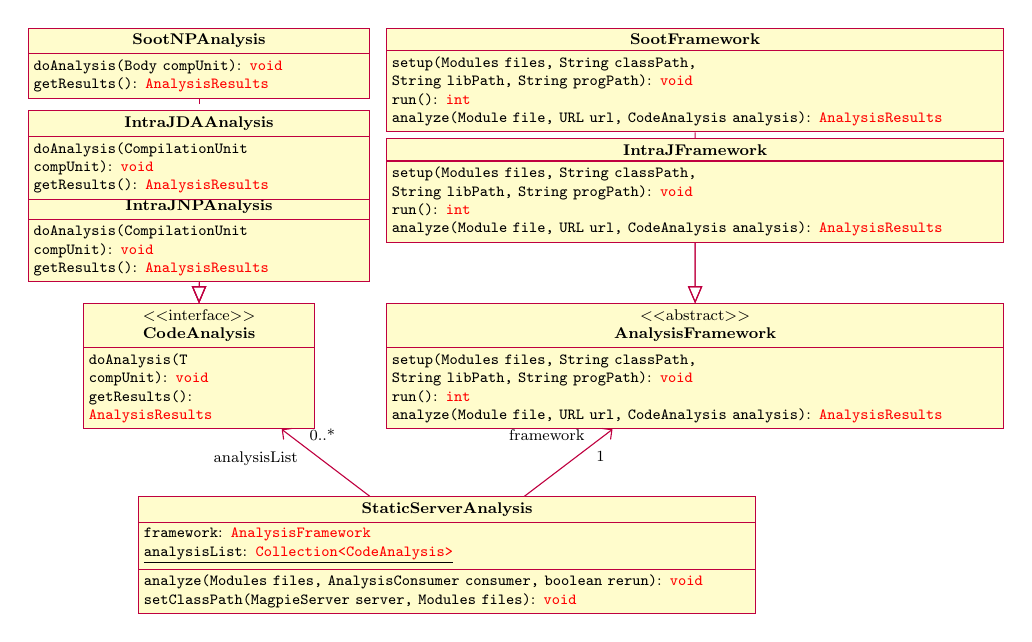
\begin{tikzpicture}[scale=0.7, every node/.style={scale=0.7}]\footnotesize
\begin{interface}[text width=4cm]{CodeAnalysis}{-3.5,-5} 
\operation{\code{doAnalysis(T compUnit)}: \code{\retType{void}}}
\operation{\code{getResults()}: \code{\retType{AnalysisResults}}} \end{interface}

\begin{abstractclass}[text width=11cm]{AnalysisFramework}{5.5,-5} 
\operation{\code{setup(Modules files, String classPath, String libPath, String progPath)}: \code{\retType{void}}}
\operation{\code{run()}: \code{\retType{int}}}
\operation{\code{analyze(Module file, URL url, CodeAnalysis analysis)}: \code{\retType{AnalysisResults}}}\end{abstractclass}

\begin{class}[text width=6cm]{IntraJNPAnalysis}{-3.5,-3} 
\implement{CodeAnalysis}
\operation{\code{doAnalysis(CompilationUnit compUnit)}: \code{\retType{void}}}
\operation{\code{getResults()}: \code{\retType{AnalysisResults}}} \end{class}

\begin{class}[text width=6cm]{IntraJDAAnalysis}{-3.5,-1.5} 
\implement{CodeAnalysis}
\operation{\code{doAnalysis(CompilationUnit compUnit)}: \code{\retType{void}}}
\operation{\code{getResults()}: \code{\retType{AnalysisResults}}} \end{class}

\begin{class}[text width=6cm]{SootNPAnalysis}{-3.5, 0} 
\implement{CodeAnalysis}
\operation{\code{doAnalysis(Body compUnit)}: \code{\retType{void}}}
\operation{\code{getResults()}: \code{\retType{AnalysisResults}}} \end{class}

\begin{class}[text width=11cm]{IntraJFramework}{5.5,-2} 
\inherit{AnalysisFramework}
\operation{\code{setup(Modules files, String classPath, String libPath, String progPath)}: \code{\retType{void}}}
\operation{\code{run()}: \code{\retType{int}}}
\operation{\code{analyze(Module file, URL url, CodeAnalysis analysis)}: \code{\retType{AnalysisResults}}}\end{class}

\begin{class}[text width=11cm]{SootFramework}{5.5,0} 
\inherit{AnalysisFramework}
\operation{\code{setup(Modules files, String classPath, String libPath, String progPath)}: \code{\retType{void}}}
\operation{\code{run()}: \code{\retType{int}}}
\operation{\code{analyze(Module file, URL url, CodeAnalysis analysis)}: \code{\retType{AnalysisResults}}}\end{class}

\begin{class}[text width=11cm]{StaticServerAnalysis}{1,-8.5} 
\attribute{\code{framework}: \code{\retType{AnalysisFramework}}}
\attribute{\underline{\code{analysisList}: \code{\retType{Collection<CodeAnalysis>}}}}
\operation{\code{analyze(Modules files, AnalysisConsumer consumer, boolean rerun)}: \code{\retType{void}}}
\operation{\code{setClassPath(MagpieServer server, Modules files)}: \code{\retType{void}}}
\end{class}

\unidirectionalAssociation{StaticServerAnalysis}{framework}{1}{AnalysisFramework}
\unidirectionalAssociation{StaticServerAnalysis}{analysisList}{0..*}{CodeAnalysis}

\end{tikzpicture}

\caption{Design structure of the source code}
\label{struct}

\end{figure*}


\subsection{Contributions}
This paper ultimately provides an implementation of an extendable source code analysis plugin for Java using \intraj\ to attain Java-specific control-flow information and \magpie\ to simplify the use of LSP and reduce the amount of code required significantly. The plugin is intended to accommodate future work to extend the analysis capabilities by adding analysis types, \jastadd\ files for \intraj\ and other analysis frameworks. The resulting extension brings the \intraj\ control flow analysis framework into a more user-friendly and accessible format that can be employed whenever an IDE has LSP support compatible with \magpie, without requiring the work overhead that comes with implementing LSP support for the extension itself. However, for this paper, only Visual Studio Code is tested and evaluated. 
\\
Also demonstrated is the increased efficiency gained from using \magpie\ by counting lines of code and comparing to the aforementioned values in Table~\ref{lsp_overhead}, which implement LSP support of their own. Additionally, the performance difference between \intraj\ and Soot is showcased, Soot being another analysis framework that does not use reference attributed grammars \cite{soot}. This is done by measuring the time for the completion of an analysis from when it starts executing in the extension until it is finished and all the results are handed over to \magpie. These measurements are done on the ANTLR 2.7.2 project, specifically the \textit{ANTLRParser.java} file. This is done to illustrate both how the extension performs on a sizable test case, and that the extension works on source code not written with the plugin in mind.
Summarizing, the contributions of this paper are the following:
\begin{itemize}
    \item A tool for finding precise analysis results efficiently using \intraj\ and providing options for quick code fixes.

    \item The implementation of an extendable framework for creating static analysis extensions for multiple IDEs through \magpie.
    
    \item Evaluation of the execution time performance of \intraj\ compared to Soot, a framework that does not use reference attributed grammars to perform its analyses.
    
    \item Demonstration of some of the utility of \magpie\ and how it affects LSP code overhead.
\end{itemize}

The rest of the paper is structured as follows. The first Section describes the implementation itself, how it works and the code structure. Section~\ref{sec:eval} discusses the evaluation process with the results of the performance evaluation and a look at the amount of code overhead generated for LSP communication. Finally, related works are discussed in Section~\ref{sec:related}.

\section{The extension}
The extension implemented is primarily targeted at performing static analyses on Java code. It is possible to extend it to support any language if supported by both the analysis framework being used and \magpie\ but currently this has not been done.
The extension framework implemented in this paper is designed to be fairly flexible. It consists of mainly two parts, one core extension framework component and one extendable custom analysis component. Figure \ref{struct} gives a brief overview of the general structure. The way it works is by defining an analysis framework and a set of code analyses to go along with it. The code analyses and analysis framework are represented by the \code{CodeAnalysis} interface and \code{AnalysisFramework} abstract class. It is then the job of a \magpie\ server analysis to define the interaction with \magpie\ and this is represented by \code{ServerAnalysis} which can be seen in Figure~\ref{struct} as well. The method for extending the analyses is determined by if the analysis framework needed is already supported or not. If it is supported then all that is needed is to write another class that implements the \code{CodeAnalysis} interface and add an instance of that class to the static \code{analysisList} in \code{ServerAnalysis}. However, if the framework is not supported the a class that extends \code{AnalysisFramework} has to be written and as of the time of writing, some minor adjustments are still needed in \code{StaticServerAnalysis} to use the new framework. After that the analysis itself can be added just as if the framework was supported initially.
\\
If \intraj\ or \extendj\ is used as AnalysisFramework it is possible to write additional \jastadd\ files for the extension that are copied over and included in the respective framework before building. This is how the string equality analysis is implemented for \intraj; a \jastadd\ file\footnote{\jastadd\ files need to be in ./src/jastadd for the pre-build copy step to work.} was written that adds an additional warning message for equality checks and a new type of warning message was added that provides more complete source code positional information. This was then leveraged to create a string equality analysis that finds these warnings and displays them.

\subsection{Performing an analysis step-by-step}

Performing an analysis and displaying the results in the IDE starts with \magpie\ and ends with \magpie. The first step is to activate one of the predefined analysis triggers. This tells \magpie\ to fetch information about which files to analyze and sends them through to the ServerAnalysis. The ServerAnalysis the uses the supplied AnalysisFramework and all active analyses (defined as CodeAnalysis types) to perform the complete analysis. This procedure follows three steps as follows.
\begin{itemize}
    \item First the AnalysisFramework is set up with any initialization that is required. For \intraj\ this means calculating all the arguments for compilation and createing a new instance of \intraj.
    \item Second the AnalysisFramework is run, performing any calculations it needs to do in order to run the analysis. \intraj\ needs to be run with the arguments from the following step to build up the graph representation of the code required for analyses.
    \item Lastly the ServerAnalysis iterates all enabled analyses and runs the AnalysisFramework dependent analysis with the currently active framework. For \intraj\ all that is needed is to find the relevant compilation units and invoke the relevant analysis method which may return warnings that are then converted to analysis results.
\end{itemize}


\begin{figure*}
    \centering
    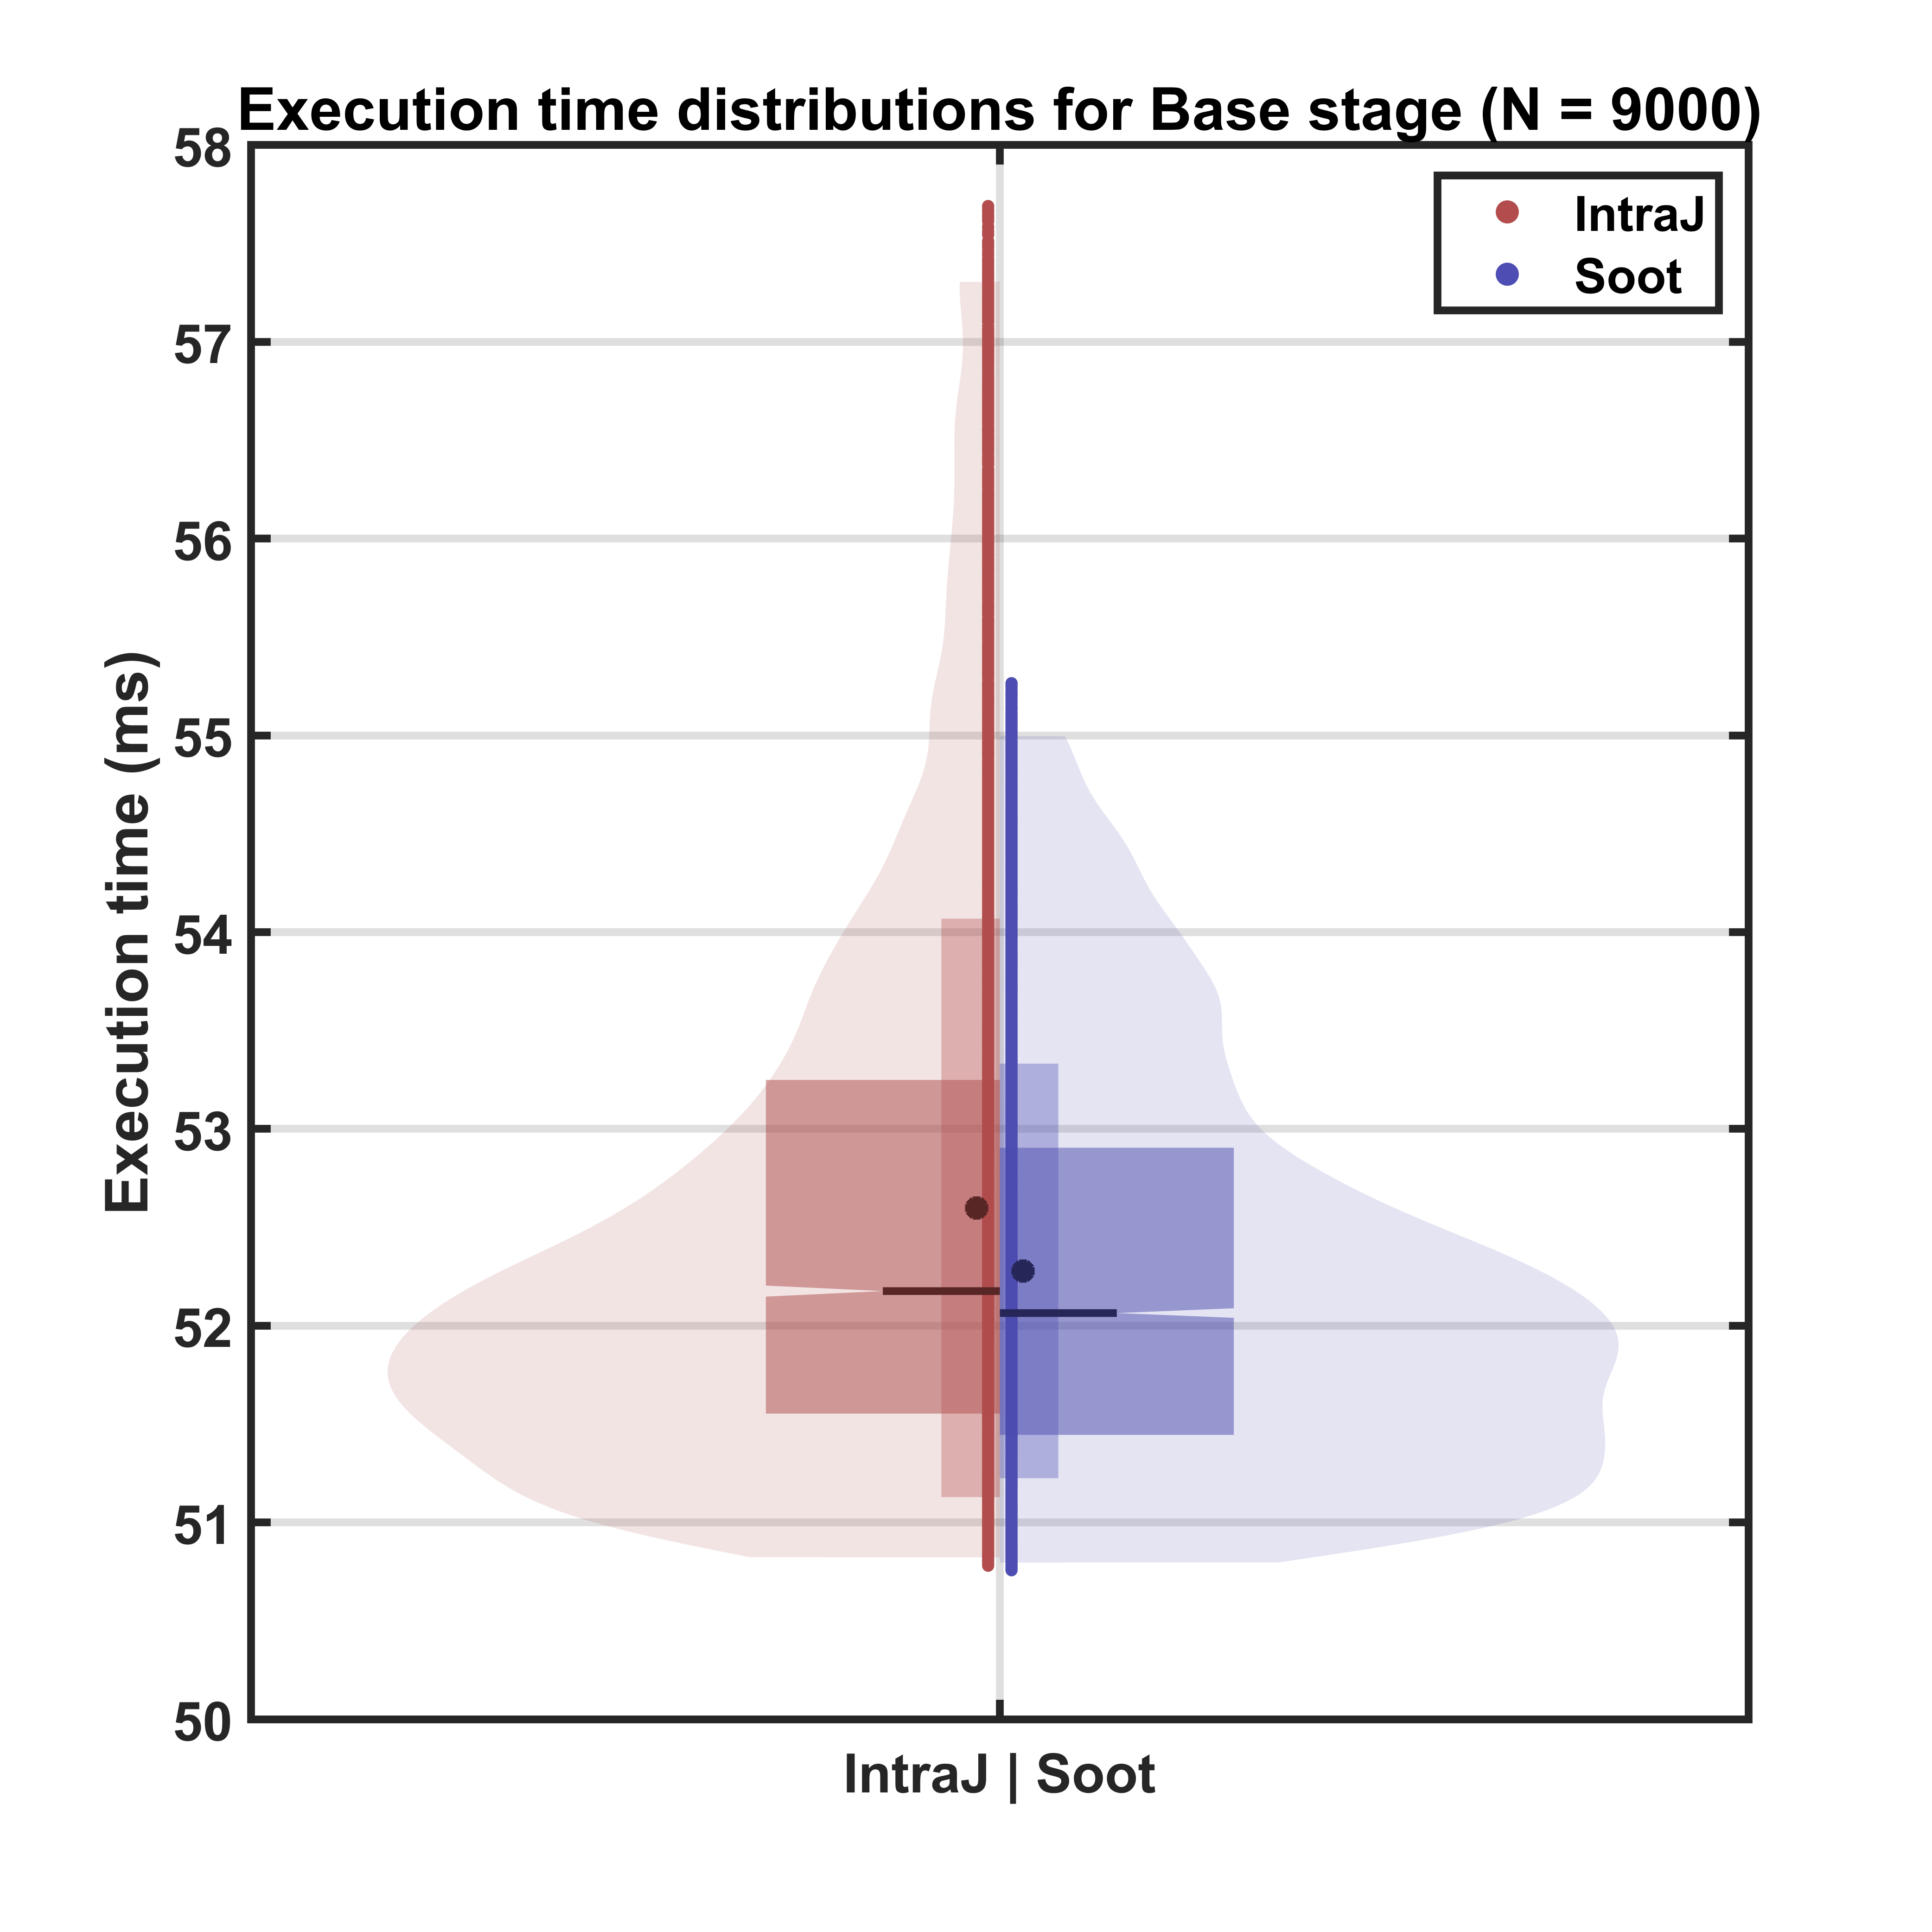
\includegraphics[width=.32\textwidth]{img/base-10000.png}\hfill
    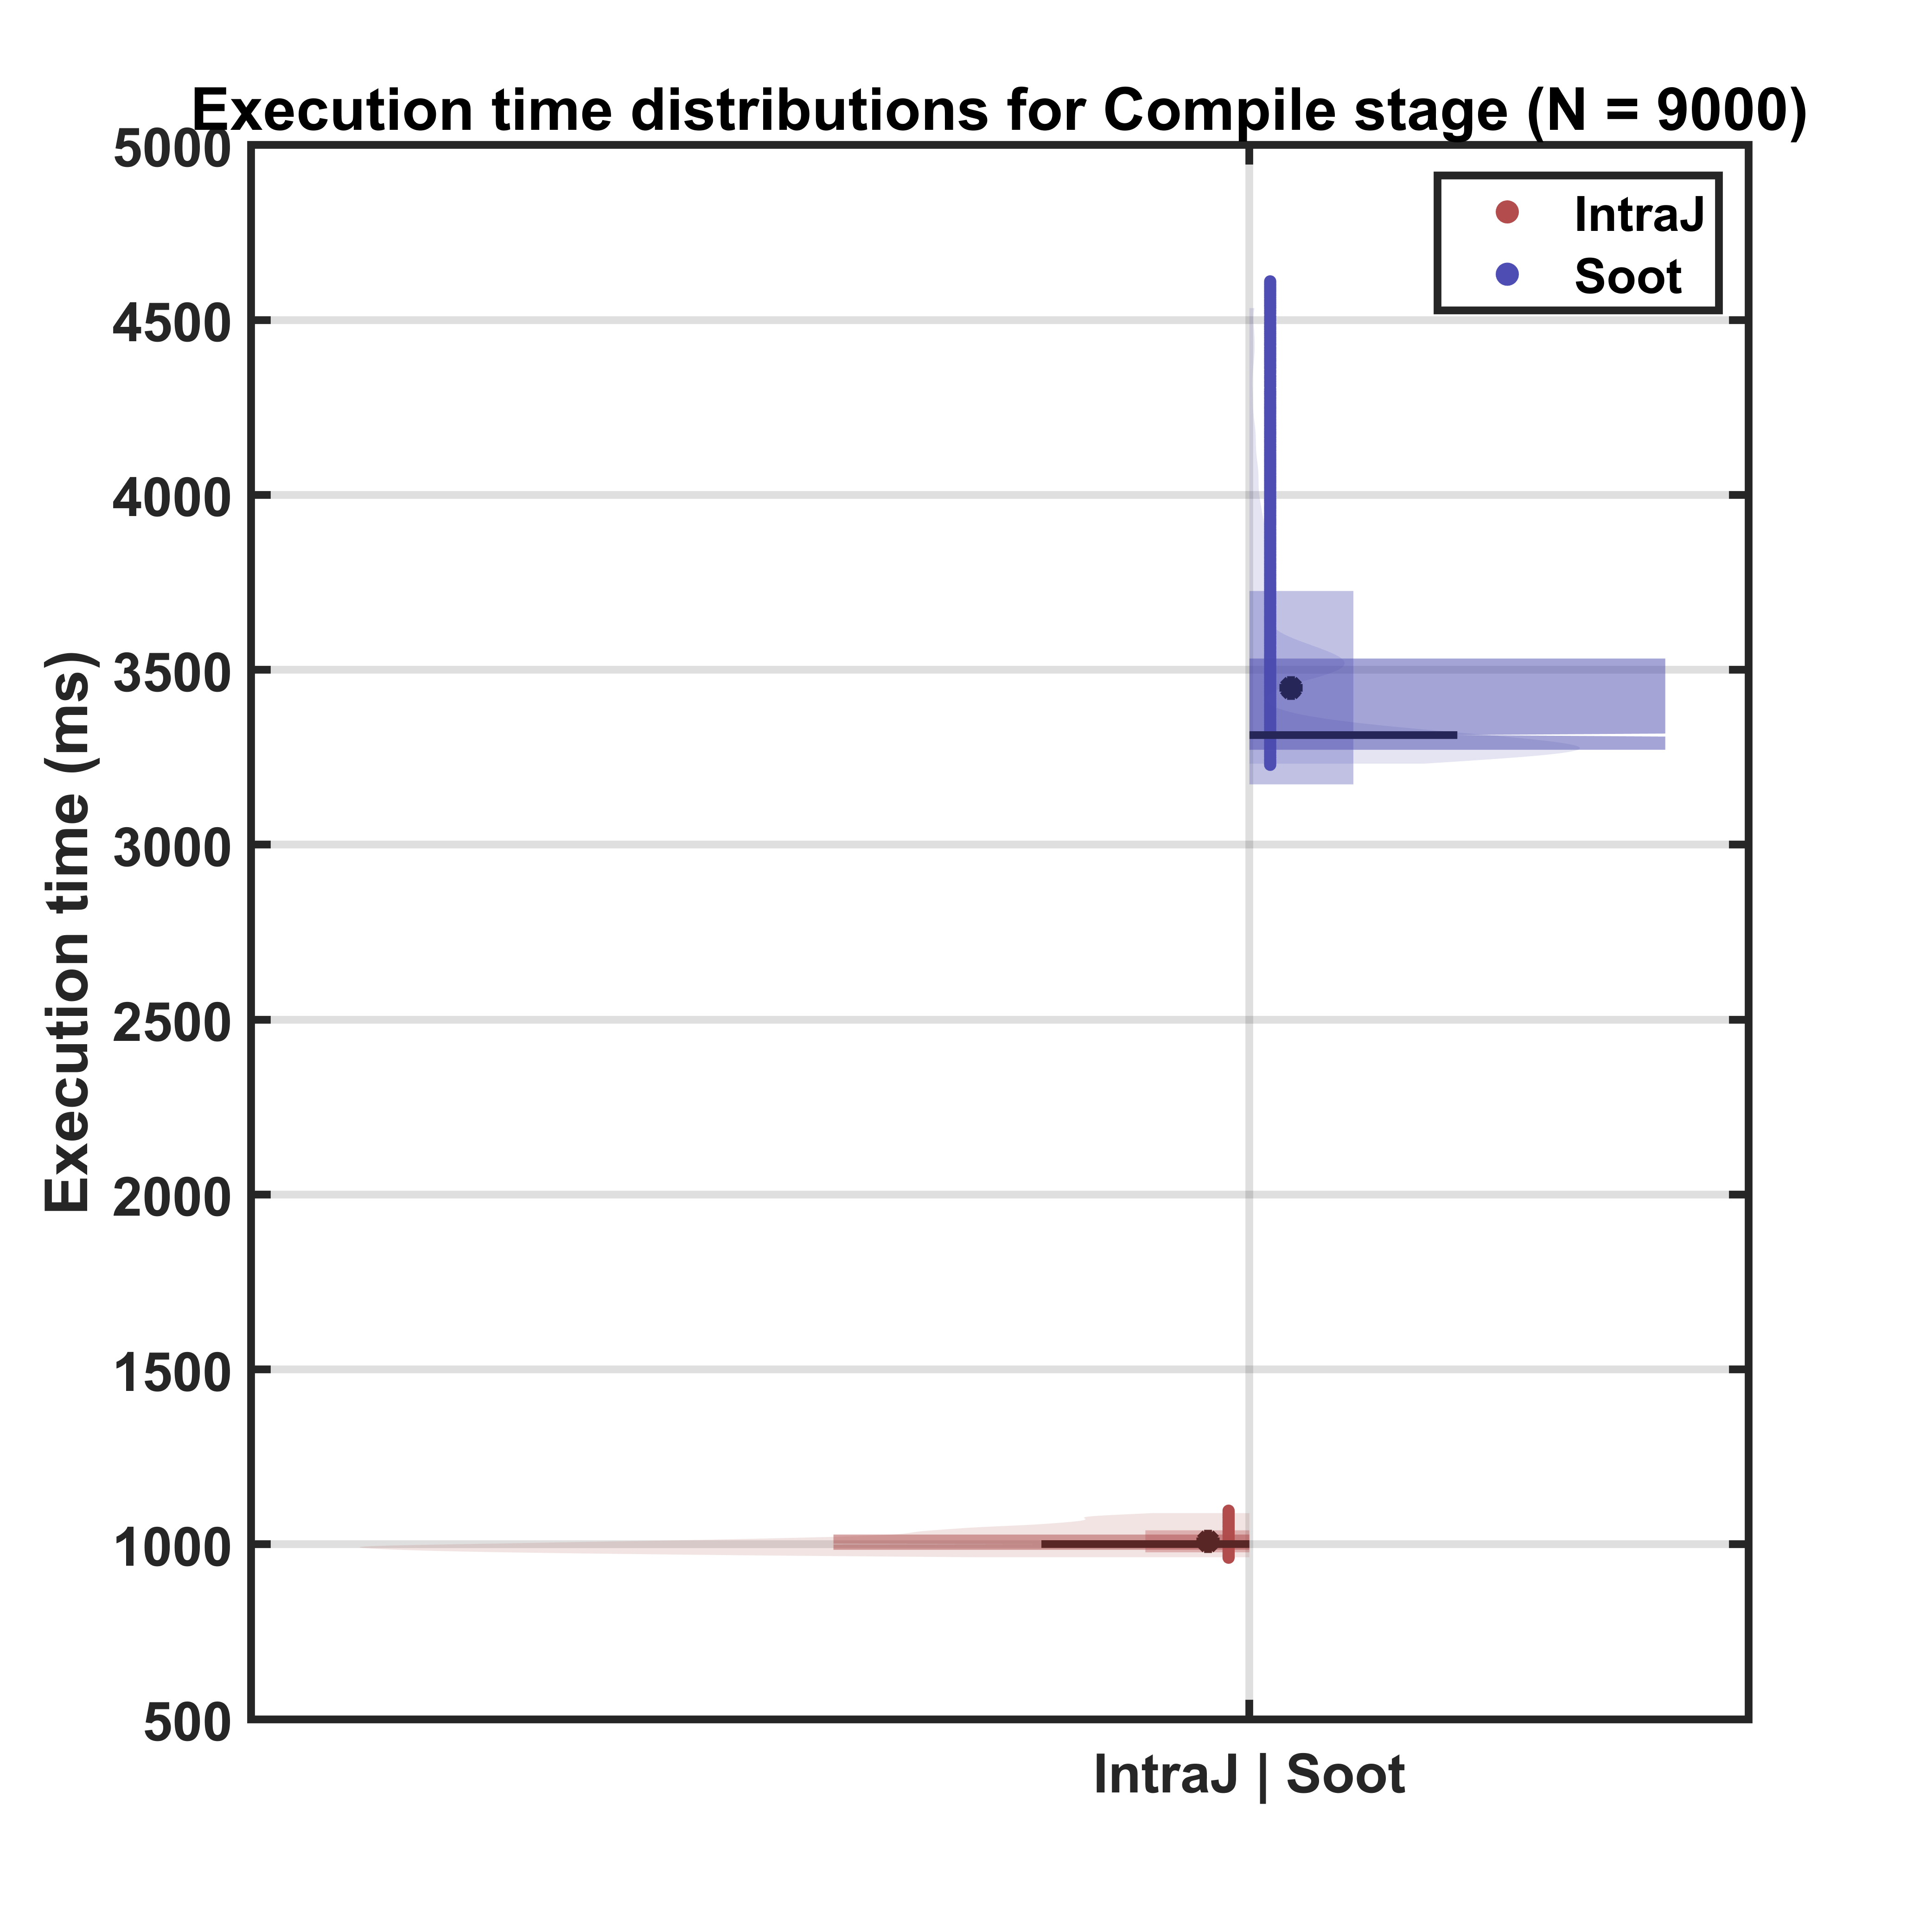
\includegraphics[width=.32\textwidth]{img/compile-10000.png}\hfill
    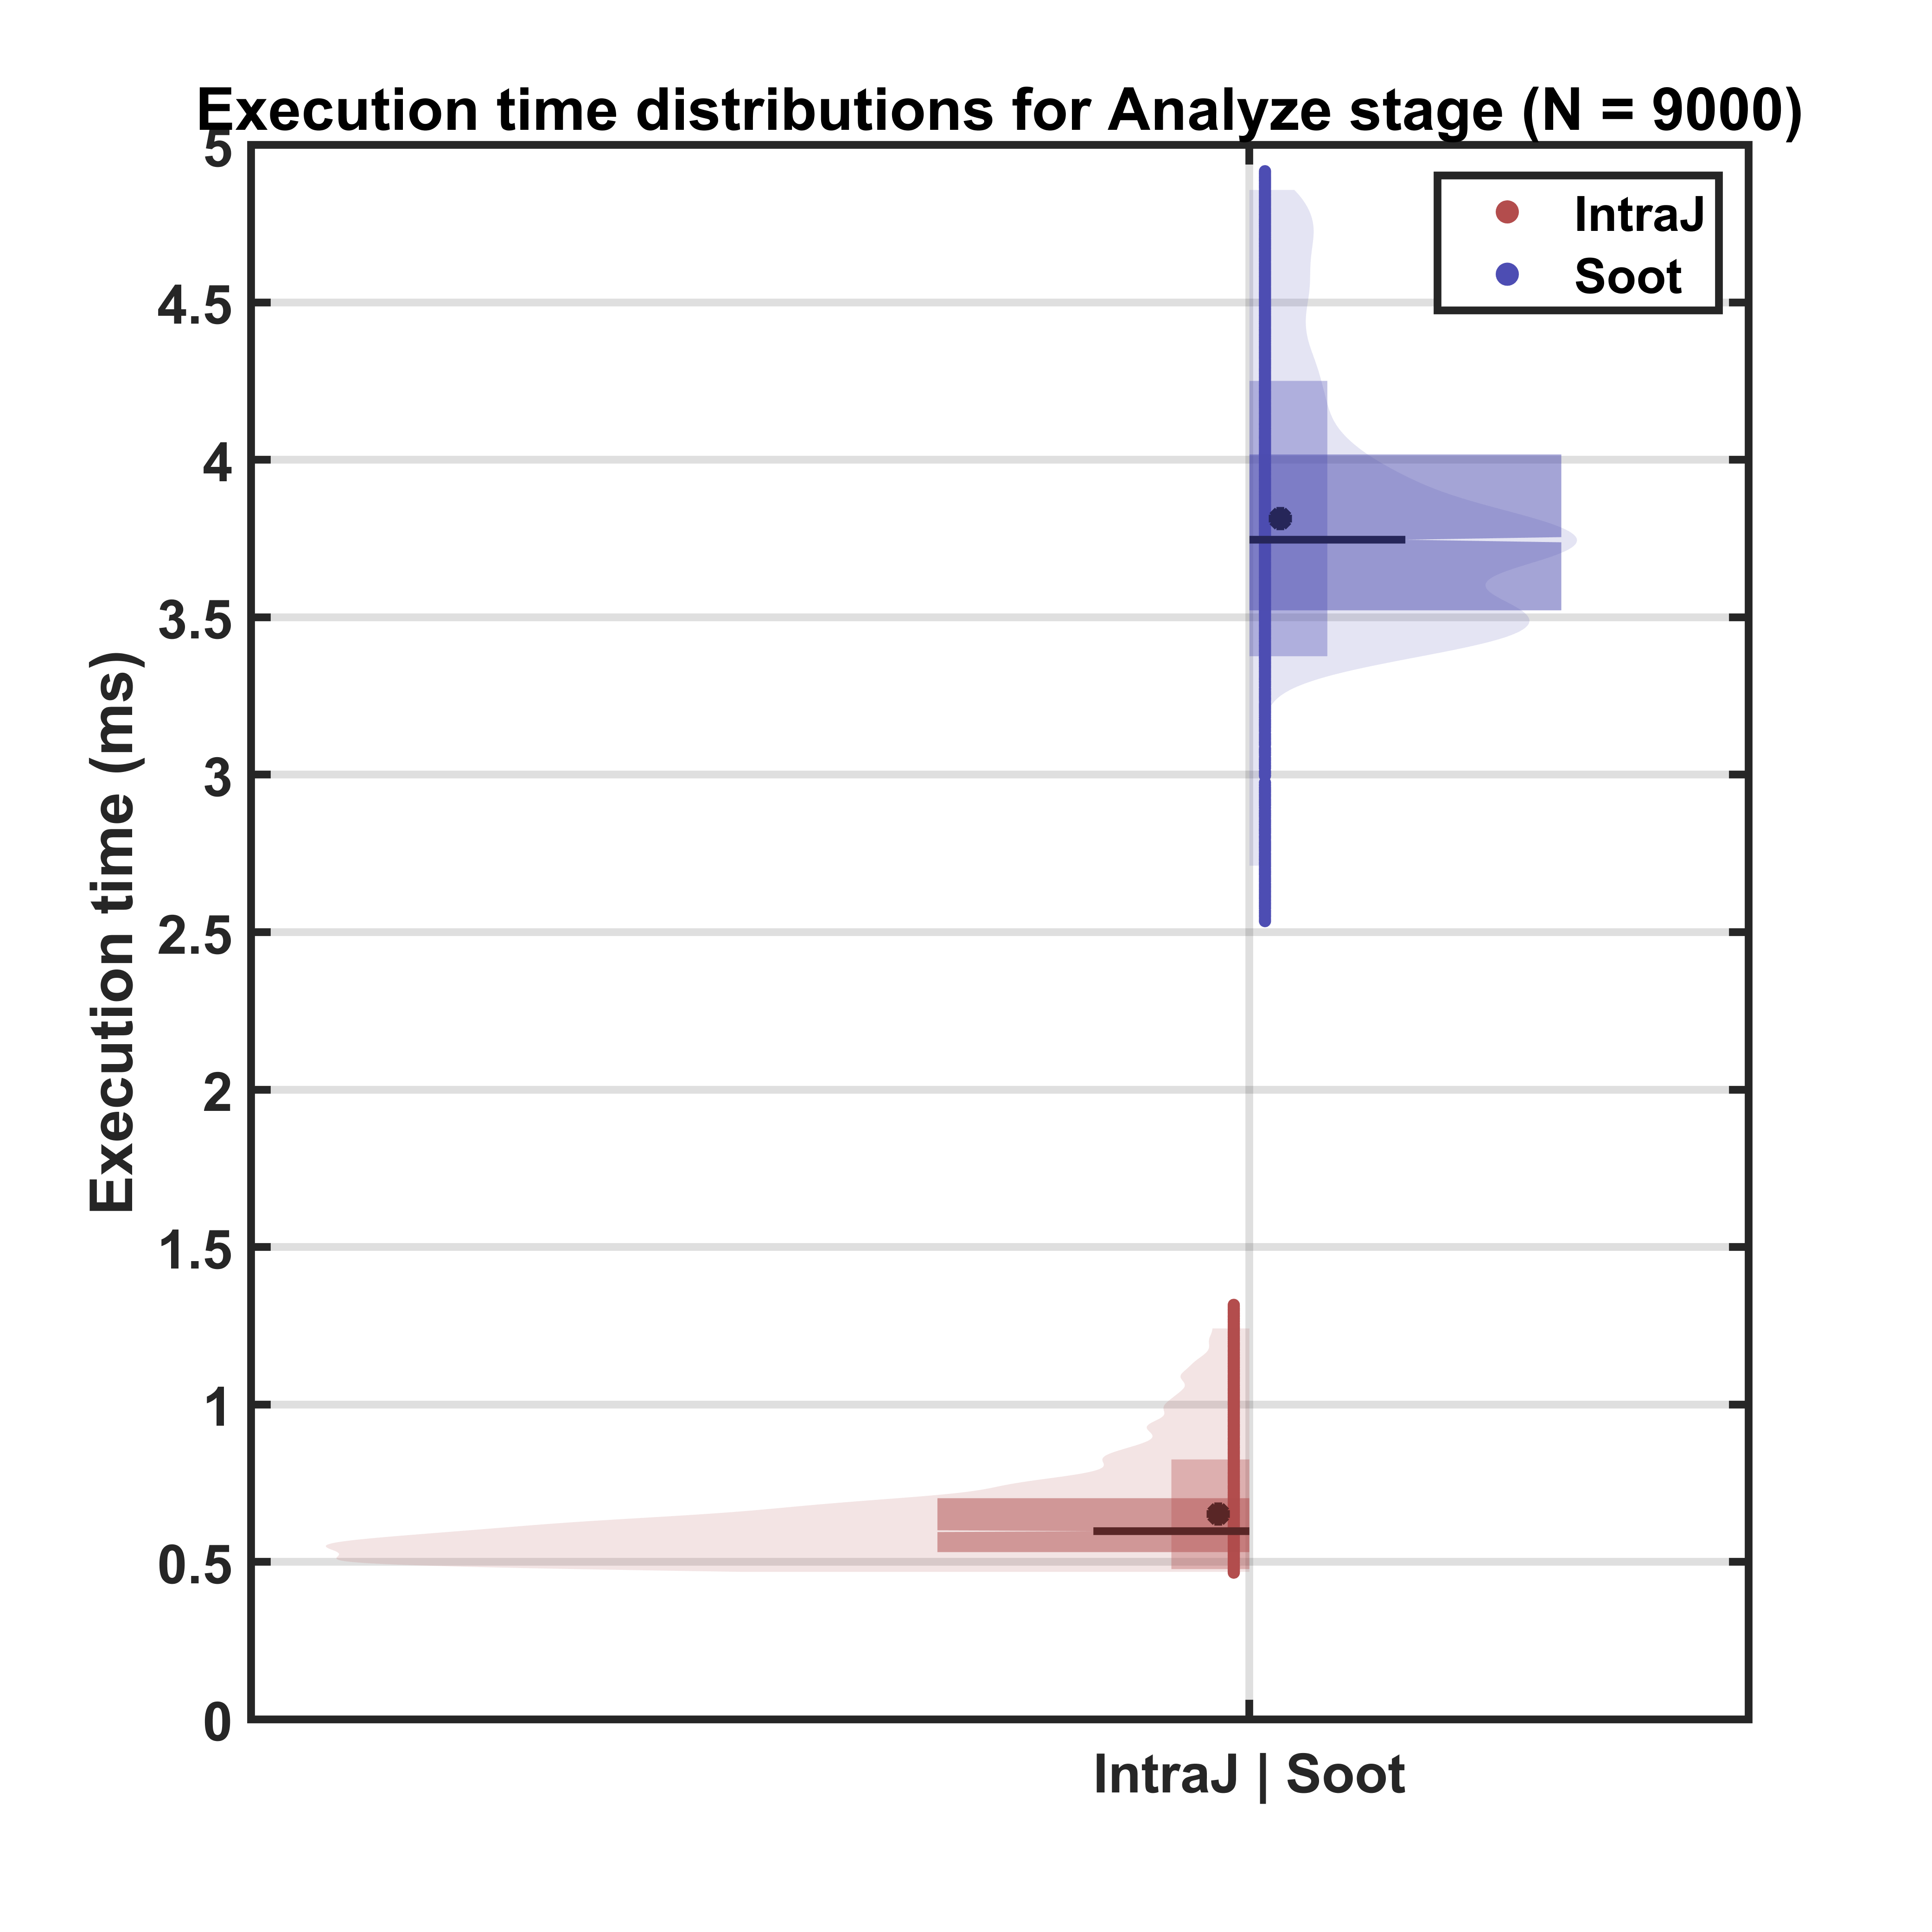
\includegraphics[width=.32\textwidth]{img/analyze-10000.png}\hfill
    \caption{Execution time results for each stage of the evaluation. From left to right you have the base, compile and analyze stage. \textbf{N} in the titles stands for the number of measurements being plotted after outliers that are more than 3 standard deviations away from the average have been eliminated. For each figure the shorter black line represents the median, the black star represents the average, the thin colored box shows one standard deviation from the average in either direction, the thick colored box with the notches represents the first and third quartiles whilst the notches represent the 95\% confidence interval around the median.}
    \label{times}
\end{figure*}

\section{Evaluation}
\label{sec:eval}
Evaluation of the extension has been performed on the metrics of source lines of code compared to other analysis extensions and analysis speed for \intraj\ and Soot  \cite{soot} using a null-pointer analysis.

\subsection{Source lines of code}
The number of lines of code excluding comments and blank lines are what will be used as the source lines of code (SLOC) metric. The implementation as of this writing contains a total of 1183 SLOC out of which 187 lines are purely used for evaluation, bringing the total SLOC used for analysis down to 996 lines. Further out of that number 75 lines come from a slightly modified file (MySourceCodeReader.java) from the \magpie\ code base that serves as a temporary fix for an issue until \magpie\ is updated. This brings the total down further to 921 SLOC. This includes code for two \intraj\ analyses, one \extendj\ analysis and one Soot analysis. \intraj\ provides a null-pointer analysis and a dead assignment analysis, \extendj\ provides a String equality analysis\footnote{Simply checks if .equals(..) or '==' is used for string operands in Java}, and Soot also provides a null-pointer analysis but based on the Soot framework instead for the purposes of comparing to \intraj.
\\
Additionally there is no code specifically meant to handle LSP communication since all of it is handled by \magpie. However, the code used to communicate with \magpie\ still had to be written which took up 375 SLOC. To compare with the values from Table~\ref{lsp_overhead} that is an overhead of $40.1\%$, in other words $40.1\%$ of the the code written for this extension is used for LSP communication, indirectly through \magpie. See Table~\ref{lsp_overhead2} for the updated version that compares this extension with the rest of the entries from before. These results puts this extension below both SPlift and CogniCrypt in terms of overhead. PMD is the only one performing better in that regard still. Note however that the code base for PMD is very big and from looking at the original table \cite{magpie} there looks to be a pattern where smaller projects suffer from worse overhead.

\begin{table}[h!]
\begin{tabularx}{\columnwidth}{brrc}
\toprule
\textsc{Tool} & \textsc{Analysis} & \textsc{Plugin} & \textsc{Overhead} (\%)\\ 
\midrule
 \texttt{SPLift} & 1$^\cdot$317 & 3$^\cdot$317 & 71.6\\
 \texttt{CogniCrypt} & 11$^\cdot$753 & 18$^\cdot$766 & 61.5\\
 \textbf{\texttt{Our extension}} & 546 & 375 & 40.1\\
 \texttt{PMD} & 117$^\cdot$551 & 33$^\cdot$435 & 22.1\\
\bottomrule
\end{tabularx}
 \caption{Updated version of Table~\ref{lsp_overhead}, now including the extension implemented in this paper.} 
 \label{lsp_overhead2}
\end{table}


\subsection{Analysis execution time}
The analysis execution time is measured by running repeated analyses on the same source files a multitude of times. After each run the time taken is recorded and another run initiated if needed. A sample size of 10000 measurements per evaluation stage was used. Important to note is that the measurements are taken 200 iterations into each run in order to avoid measuring the start-up times and instead measure steady-state times, which should be more representative of actual usage of the extension over a period of time. The only source file used to run the evaluation is  \textit{ANTLRParser.java} from ANTLR 2.7.2\footnote{https://www.antlr.org/}. The analysis is specifically performed on Visual Studio Code, as this is the only IDE this extension has been tested on. Soot \cite{soot} was chosen to compare against \intraj\ due to Soot being a well known and established analysis framework and to try and illustrate some of the performance differences between using a reference attributed grammar (\intraj) and not doing so. The computer used to run the evaluation is a Lenovo Thinkpad T460s and it has the following hardware specifications.

\begin{itemize}
    \item CPU: Intel Core i5-6300U, 2.4 GHz
    \item OS: Windows 10 Pro 64-bit
    \item RAM: 16 GB DDR4
    \item Graphics: Intel HD Graphics 520
    \item Storage: 128 GB SSD, SAMSUNG MZNTY128HDHP-000L1
\end{itemize}

\\
The evaluation happens in three stages, dubbed Base, Compile and Analyze. The Base stage runs no framework functionality at all and is the same across both \intraj\ and Soot. What is measured in Base consists of all background code that supports the analysis, most notably the calculation of the analyzed projects source paths, library paths and class path. This calculation will take a long time first time it is run due to \magpie\ initiating a project service. Therefore the project service initiation is done separately before evaluation begins in the interest of keeping the measurements fair for both frameworks. The Compile stage runs everything from the Base stage and also runs all the setup code required for the framework to run analyses. For \intraj\ this means parsing the relevant code into an abstract syntax tree (AST) and inserting the control-flow attributes where they are needed. In the case of Soot a conversion from the internal representations (IR) used by Wala to the Jimple IR used by Soot is required. The time measured for the Compile stage is only the framework setup code, specifically \code{setup(...)} and \code{run()} methods from the \code{AnalysisFramework} class in Figure~\ref{struct} The Analyze stage runs everything from the Compile stage and additionally runs a null-pointer exception analysis. For \intraj\ the built-in null-pointer analysis is used while for Soot a custom made forward analysis is used. This custom made analysis is based on a sample implementation made by Navid Salehnamadi\footnote{\url{https://github.com/noidsirius/SootTutorial}} and may not be optimal, however given how simple the analysis is it is hard to imagine how to improve on execution time without changing the underlying Soot code or something similar. The time measured for the Analyze stage is only the time it takes from starting the analysis thread which runs the analysis until that thread has finished.
\\
The results of the comparison for each stage outlined above is visualized in Figure~\ref{times}. Seemingly IntraJ perfoms much faster with the Analyze stage median execution time being around $0.5$ ms whilst Soot measures in at around $4$ ms. However, the biggest performance load for Soot seems to come from the Compile stage and after further investigation and profiling the code using JProfiler 12.0.4 it turns out that the majority of the Compile stage is spent converting the Wala IR into Jimple. Further it turns out that the bad performance is mostly due to a large number of instantiations of temporary objects done in the Wala source code. In other words, this is not intrinsically due to how Soot operates but due to the fact that \magpie\ requires a conversion to use Soot analyses.

The Base evaluation stage displayed to the left in Figure~\ref{times} is largely the same for both \intraj\ and Soot as expected since this stage is independent of any analyses and analysis frameworks. Both frameworks the Base stage results have a median of about $50$ ms which means that the supporting extension code outside of the framework and analysis specific code takes around that long to execute. 

\section{Related work}
\label{sec:related}
Previous attempts at bringing the various errors and warnings from \extendj\ into the IDE using LSP have been made in the past as part of similar projects to the one presented in this paper \cite{old1, old2}. These older attempts managed to implement  LSP support to display diagnostic messages over the code in-editor and showcased how their extensions then could display \extendj\ errors and warnings in a handful of IDEs. The extension implemented for this paper performs a similar function in that it displays some warnings, however for the purposes of this paper no \extendj\ native warnings or errors are considered\footnote{The string equality check is not being considered native as it stems from an extension made to \extendj}. The biggest difference between the work done in those previous attempts and this one is the use of \magpie\ to abstract the LSP support away from the extension itself. This has provided many benefits such as out-of-the-box ready LSP features that can be used without needing to know the technical details of LSP and simplified extension building for multiple IDEs that can be provided by \magpie\ and does not require the developer to figure out how to build for a particular IDE. For example, the Visual Studio Code extension building script used to build the extension was provided by \magpie, and the quick fix IDE prompts were part of the \magpie\ analysis result handling code. Another addition that sets this work apart from the previous is that the results displayed can be powered not only by \extendj\ but also by \intraj, Soot and other analysis frameworks or compilers.

\section{Conclusion}

From the evaluation results we can draw two main conclusions. First, the SLOC count results seems to indicate that the workload for implementing LSP support is indeed smaller when using \magpie. This is not strong evidence for this feature of \magpie\ as not enough cases are considered and this project is not of commercial scale by any means. But with more research and application of LSP abstracting frameworks such as \magpie\ the picture might become clearer. 
\\
Secondly, the execution time of \intraj\ does seem to be smaller than that of Soot. Focusing only on the Analyze stage results, they seem to paint a promising picture of \intraj\ efficiency in performing static intraprocedural analysis. It is however important to bear in mind that these results are derived from evaluating the performance on a single project (ANTLR 2.7.2), on a single file within said project (\textit{ANTLRParser.java}), using only a single analysis (Null-pointer analysis). There is no guarantee that \intraj\ will remain faster when more files, projects and analyses are considered. Another important distinction between \intraj\ and Soot is that unlike \intraj, Soot allows for more than just intraprocedural analysis. In addition to intraprocedural analysis Soot provides functionality to do interprocedural analysis as well as transforming the byte code for optimization purposes. Yet another consideration to be made is that the speed difference observed between Soot and \intraj\ is definitely attributable to RAGs on-demand evaluation feature. More controlled tests would be needed to determine this.
\\
Finally as an additional note it should be mentioned that the Compile stage execution times could potentially be improved for \intraj. Right now the Compile stage code runs \intraj\ on the full project, classpath, source files, and libarary files included. For the purposes of intraprocedural analysis technically only the file to be analyzed needs to be examined, however this would most likely produce compilation errors wiht \intraj. If those compilation errors are ignored and the AST is built with all CFG attributes present, then \intraj\ should still be able to run the analyses required. Doing this could improve the Compile stage times for \intraj\ considerably and more importantly it would decouple the Compile stage code execution time from the project size, instead only depending on the individual file size to be analyzed. This could be part of some future work done on this extension. Other work that can still be done would include extending the analysis suite to support more types of analyses, extending the number of supported analysis frameworks, including a \code{AnalysisFramework} reference in \code{CodeAnalysis} so that the \code{StaticServerAnalysis} class does not have to know about the \code{AnalysisFramwork} and can thus perform analyses regardless of which framework they belong to since all framework related information is embedded in the analysis class. Also for the evaluation, there is a lot of work to be done still; evaluating on other projects and files and doing more controlled tests that can better determine where performance differences arise would be the two most prominent places to start.

%% Acknowledgments
\begin{acks}
I would like to thank my supervisor Idriss Riouak for his patient guidance and help with troubleshooting.
\end{acks}


%% Bibliography
\bibliography{bib}

\end{document}
